\appendix
\onecolumn
\section{Codes}
\subsection{\texttt{std::bitset} vs \texttt{std::set}}
\label{app:setbench}
\begin{verbatim}

#define N 65
#define SIZE 32*N

static std::set<uint16_t>* copy(const std::bitset<SIZE>* a) {
    std::set<uint16_t>* res = new std::set<uint16_t>;
    for (uint16_t i = 0; i < SIZE; i++) {
        if (a->test(i)) res->insert(i);
    }
    return res;
}

int main() {
    srand((unsigned int)time(NULL));

    std::vector<std::bitset<SIZE>*> bitsets;

    for (int i = 0; i < 3000; i++) {
        std::stringstream ss;
        for (int j = 0; j < N; j++) {
            std::bitset<32> bs(rand());
            ss << bs.to_string();
        }
        bitsets.push_back(new std::bitset<SIZE>(ss.str()));
    }

    std::vector<std::set<uint16_t>*> sets;
    for (int i = 0; i < 3000; i++) {
        sets.push_back(copy(bitsets[i]));
    }

    bool fool;

    double t1 = omp_get_wtime();
    for (uint16_t i = 0; i < sets.size(); i++) {
        for (uint16_t j = 0; j < sets.size(); j++) {
            fool = isSubset(*sets[i], *sets[j]);
        }
    }
    double t2 = omp_get_wtime();

    for (uint16_t i = 0; i < bitsets.size(); i++) {
        std::bitset<SIZE> notb = ~(*bitsets[i]);
        for (uint16_t j = 0; j < bitsets.size(); j++) {
            fool = isSubset_bit(notb, *bitsets[j]);
        }
    }
    double t3 = omp_get_wtime();

    std::cout << "(" << SIZE << ", " << (t2-t1) << ")\n";
    std::cout << "(" << SIZE << ", " << (t3-t2) << ")\n";
}

\end{verbatim}

\subsection{next\_combination}
\label{app:nextcombination}
\begin{verbatim}
template <class BidIt>
inline bool next_combination(BidIt n_begin, BidIt n_end, BidIt r_begin, BidIt r_end)
{
    bool boolmarked=false;
    BidIt r_marked;

    BidIt n_it1=n_end;
    --n_it1;


    BidIt tmp_r_end=r_end;
    --tmp_r_end;

    for(BidIt r_it1=tmp_r_end; r_it1!=r_begin || r_it1==r_begin; --r_it1,--n_it1)
    {
        if(*r_it1==*n_it1 )
        {
            if(r_it1!=r_begin) //to ensure not at the start of r sequence
            {
                boolmarked=true;
                r_marked=(--r_it1);
                ++r_it1;//add it back again 
                continue;
            }
            else // it means it is at the start the sequence, so return false
                return false;      
        }
        else //if(*r_it1!=*n_it1 )
        {
            //marked code
            if(boolmarked==true)
            {
                //for loop to find which marked is in the first sequence
                BidIt n_marked;//mark in first sequence
                for (BidIt n_it2=n_begin;n_it2!=n_end;++n_it2)
                    if(*r_marked==*n_it2) {n_marked=n_it2;break;}


                BidIt n_it3=++n_marked;    
                for  (BidIt r_it2=r_marked;r_it2!=r_end;++r_it2,++n_it3)
                {
                    *r_it2=*n_it3;
                }
                return true;
            }
            for(BidIt n_it4=n_begin; n_it4!=n_end; ++n_it4)
                if(*r_it1==*n_it4)
                {
                    *r_it1=*(++n_it4);
                    return true;           
                }
        }
    }  

    return true;//will never reach here    
}
\end{verbatim}

\twocolumn

\begin{comment}
\chapter{Example Tree of Some $\mathcal{Q}$}
\label{app:tree}
\centering
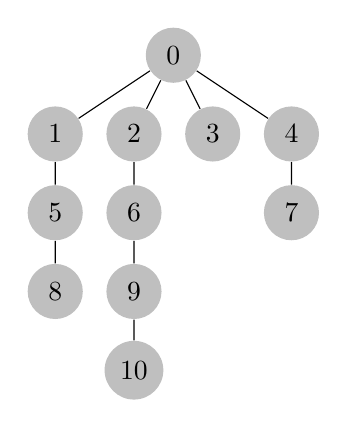
\begin{tikzpicture}[level/.style={sibling distance=10mm/#1, level distance=10mm}]
\tikzset{every node/.style={shape=circle,fill=black!25,minimum size=7mm}}
%\tikzset{every node/.style={shape=circle,
%                            font=\bfseries \Large,
%                            minimum size=3cm,
%                            scale=0.4
%                           }}
\node (root) {$0$}
    child {
        node {$1$}
        child {
            node (n5) {$5$}
            child {
                node {$8$}
            }
        }
    }
    child {node (n2) {$2$}
        child {node (n6) {$6$}
            child {node {$9$}
                child {node {$10$}
                }
            }
        }
    }
    child {node (n3) {$3$}
    }
    child {node (n4) {$4$}
        child {node {$7$}
        }
    }
    ;
\end{tikzpicture}


\chapter{Slp Header Files}

\section*{\texttt{Algorithm.hpp}}
\begin{verbatim}
/**
 * Perform a line search by finding the minimum objective value
 * of the given QP problem of all the points between the two
 * given points.
 *
 * @param  p1
 *         Start point.
 * @param  p2
 *         End point.
 * @param  model
 *         ClpModel of the QP problem.
 * @return the step length alpha.
 */
double lineSearch(double* p1, double* p2, const ClpModel model);
\end{verbatim}

\begin{verbatim}
/**
 * Solve a QP problem using Slp.
 *
 * @param  quad
 *         ClpModel containing the QP problem.
 * @param  x
 *         Array containing the initial guess vector. This array
 *         will be overwritten with a final solution.
 * @param  maxIters
 *         Number of iterations to perform if the stopping
 *         criteria is not met.
 * @param  tol
 *         Epsilon for the stopping criteria.
 * @return the objective value of the solved QP problem..
 */
double solve(ClpModel quad, double* x, int maxIters, double tol);
\end{verbatim}

\begin{verbatim}
/**
 * Perform a Taylor-series expansion of the objective function of
 * the given QP problem at the given point.
 *
 * @param destCoeffs
 *        Pointer to coefficient destination.
 * @param point
 *        Point to perform the expansion at.
 * @param model
 *        ClpModel that has the objective function.
 */
void taylor(double* destCoeffs, double* point, ClpModel model);
\end{verbatim}

\begin{verbatim}
/**
 * Evaluate the objective function of the given model at
 * the given point.
 *
 * @param point
 *        Point to evaluate the objective function at.
 * @param model
 *        ClpModel that has the objective function to evaluate.
 */
doubld value(double* point, ClpModel model);
\end{verbatim}
\end{comment}
